\documentclass[twoside]{article}
\usepackage[T1,T2A]{fontenc}
\usepackage[utf8]{inputenc}
\usepackage[french,english,russian]{babel}
\usepackage[pdftex]{graphicx}
\usepackage{cmap}
\usepackage{hyperxmp}
\usepackage[colorlinks,linkcolor=blue]{hyperref}
\usepackage[landscape,left=0.1cm, right=.1cm, top=0.1cm, bottom=.1cm,paperwidth=7in,paperheight=9in]{geometry}

\usepackage[dvipsnames]{xcolor}
\usepackage{tikz}
\usepackage{calc}
\usetikzlibrary{shapes.misc}
\usetikzlibrary{mindmap}

\usepackage{varwidth}
\usepackage{fancyhdr}
\usepackage{chronosys}

\renewcommand{\headrulewidth}{0pt}
\renewcommand{\footrulewidth}{0pt}

\newcommand{\myhref}[2]{\selectlanguage{french}\textcolor{blue}{\href{#1}{\selectlanguage{russian}\textcolor{blue}{#2}}}\selectlanguage{russian}}

\author{Vitaly Repin \thanks{Thanks to Prof. Michael S. Roth, Wesleyan University and Coursera}}
\title{The Modern and the Postmodern\\  \textit{\small Visual arts discussed in the course on the Modern and the Postmodern @ Wesleyan University}}
\date{September 2013}

\hypersetup{%
pdftitle={%
The Modern and the Postmodern. Visual arts discussed in the course on the Modern and the Postmodern @ Wesleyan University},
pdfauthor={Vitaly Repin},
pdfauthortitle={Coursera student},
pdfcopyright={This work is licensed under a Creative Commons Attribution-ShareAlike 3.0 Unported License},
pdfsubject={The Modern and the Postmodern},
pdfkeywords={modern,postmodern,mante,courbet,delacroix},
pdflicenseurl={http://creativecommons.org/licenses/by-sa/3.0/},
pdfcaptionwriter={Vitaly Repin},
pdfcontactcity={Espoo},
pdfcontactcountry={Finland},
pdfcontactemail={vitaly.repin@gmail.com},
pdflang={en}
}


\begin{document}
\maketitle
\newpage

%% From Locke to Freud: mindmap
%% From Locke to Freud: mindmap
\thispagestyle{sideheadingnowiki}
\pdfbookmark[2]{From Locke to Freud: Art, Philosophy, Science and History. Mindmap}{Lock2Freud}
\phantomsection
\addcontentsline{toc}{section}{From Locke to Freud: Art, Philosophy, Science and History. Mindmap}

\hspace*{1cm}\copyrightboxOddEven{%
\begin{tikzpicture}[scale=0.95,mindmap,
every node/.style={concept,execute at begin node=\hskip0pt},
root concept/.append style={
concept color=black, fill=white, line width=1ex, text=black,minimum size=3cm,text width=3cm,font=\large\scshape},
text=historyfg,
concept color=historybg,grow cyclic,
level 1/.append style={level distance=3.7cm,sibling angle=90},
level 2/.append style={level distance=3cm,sibling angle=45},
level 3/.append style={level distance=2.3cm,sibling angle=45}]
\node[root concept] {Modernity: From Locke to Freud}
  child [concept,sibling angle=95,color=historybg,text=historyfg] { node {History}
	child[sibling angle=50] { node {Germany}
		child { node {\hrefmm{http://en.wikipedia.org/wiki/Unification_of_Germany}{historyfg}{1871: Unification of Germany}}}
		child { node {\hrefmm{http://en.wikipedia.org/wiki/Austro-Prussian_War}{historyfg}{1866: Austro-Prussian War}}}
		child { node {\hrefmm{http://en.wikipedia.org/wiki/Second_Schleswig_War}{historyfg}{1864: Second Schleswig War}}}
	}
	child[sibling angle=67] { node {England} 
		child { node {\hrefmm{http://en.wikipedia.org/wiki/Glorious_Revolution}{historyfg}{1688 -- 1689: Glorious Revolution}}}
	}
	child[sibling angle=72,level distance=3.8cm] { node {France} 
		child { node {\hrefmm{http://en.wikipedia.org/wiki/Haussmann\%27s_renovation_of_Paris}{historyfg}{1853--1870: Hauss\-mann's renovation of Paris}}}
		child { node {\hrefmm{http://en.wikipedia.org/wiki/June_Days_Uprising}{historyfg}{1848: June Days Uprising}}}
		child { node {\hrefmm{http://en.wikipedia.org/wiki/Revolutions_of_1848_in_France}{historyfg}{1848: French Revolution of 1848}}}
		child { node {\hrefmm{http://en.wikipedia.org/wiki/Louis_Philippe_I}{historyfg}{1830--1848: Louis Philippe}}}
		child { node {\hrefmm{http://en.wikipedia.org/wiki/Reign_of_Terror}{historyfg}{1793--1794: Reign of Terror}}}
		child { node {\hrefmm{http://en.wikipedia.org/wiki/French_revolution}{historyfg}{1789: French Revolu\-tion}}}
	}
	child[sibling angle=70] { node {Europe} 
		child { node {\hrefmm{http://en.wikipedia.org/wiki/Vienna_congress}{historyfg}{1814--1815: Congress of Vienna}}}
		child { node {\hrefmm{http://en.wikipedia.org/wiki/Franco-Prussian_War}{historyfg}{1870--1871: Franco-Prussian War}}}
		child { node {\hrefmm{http://en.wikipedia.org/wiki/World_War_I}{historyfg}{1914-1918: World War I}}}
	}	
  }
  child [concept color=scibg,text=black,sibling angle=70] { node {Science}
	child { node {\hrefmm{http://en.wikipedia.org/wiki/On_the_Origin_of_Species}{black}{1859: On the Origin of Species}}}
	child { node {\hrefmm{http://en.wikipedia.org/wiki/Descent_of_man}{black}{1871: The Descent of Man}}}
	child { node {\hrefmm{http://en.wikipedia.org/wiki/The_Interpretation_of_Dreams}{black}{1899: The Interpre\-tation of Dreams}}}
  }
  child [concept color=historybg,text=historyfg,level distance=5cm] { node { Philosophy}
  	child { node {\hrefmm{http://en.wikipedia.org/wiki/Civilization_and_Its_Discontents}{historyfg}{1930: Civilization and Its Discontents}}}
	child { node {\hrefmm{http://en.wikipedia.org/wiki/On_the_Genealogy_of_Morals}{historyfg}{1887: On the Genealogy of Morality} }}
	child { node {\hrefmm{http://en.wikipedia.org/wiki/The_Communist_Manifesto}{historyfg}{1848: The Communist Manifesto} }}
	child { node {\hrefmm{http://en.wikipedia.org/wiki/Answering_the_Question:_What_is_Enlightenment\%3F}{historyfg}{1784: What is Enlighten\-ment?}}}
	child { node {\hrefmm{http://en.wikipedia.org/wiki/Discourse_on_the_Origin_of_Inequality}{historyfg}{1755: Discourse on Inequality}}}
	child[sibling angle=48] { node {\hrefmm{http://en.wikipedia.org/wiki/Discourse_on_the_Arts_and_Sciences}{historyfg}{1750: Discourse on the Arts and Sciences}}}
  }
  child [concept color=scibg,text=black] { node {Arts}
  	child [concept, sibling angle=70 ] { node {Literature}
  		child { node {\hrefmm{http://en.wikipedia.org/wiki/Paris_Spleen}{black}{1869: Le Spleen de Paris}}}
		child { node {\hrefmm{http://en.wikipedia.org/wiki/Madame_Bovary}{black}{1856: Madame Bovary}}}
  	}
	child [concept ] { node {Paintings}
		child[sibling angle=40] { node {\hrefmm{http://en.wikipedia.org/wiki/Impressionism}{black}{Impres\-sionism}}
  			child { node {\hrefmm{http://en.wikipedia.org/wiki/Olympia_(Manet)}{black}{1863: Olympia } }}
		}
		child { node {\hrefmm{http://en.wikipedia.org/wiki/Realism_(visual_arts)}{black}{Realism}}
			child { node {\hrefmm{http://en.wikipedia.org/wiki/The_Stone_Breakers}{black}{1850: The Stone Breakers}}}
		}
		child[sibling angle=35] { node {\hrefmm{http://en.wikipedia.org/wiki/Romanticism}{black}{Romantis\-cism}}
			child [sibling angle=55] { node {\hrefmm{http://en.wikipedia.org/wiki/Liberty_Leading_the_People}{black}{1830: Liberty Leading the People } }}
			child[sibling angle=60] { node {\hrefmm{http://en.wikipedia.org/wiki/The_Massacre_at_Chios}{black}{1824: The Massacre at Chios} }}
		}
		child[sibling angle=37] { node {\hrefmm{http://en.wikipedia.org/wiki/Neoclassicism}{black}{Neoclas\-sicism}} }
  	}
  };
\end{tikzpicture}}




%% Paintings
%% Paintings
\addcontentsline{toc}{section}{Paintings of the Modern}

\pagestyle{sideheading}

\newcommand{\pictitle}[6]{\addcontentsline{toc}{subsection}{#1 (#2)}%
\myhref{#6}{\textsf{\textbf{#1 (#2, #3).}}} \textit{#4.} #5.\bigskip}

\newenvironment{myframe}{\begin{center}}{\end{center}\newpage}

\newcommand{\pict}[1]{\includegraphics[keepaspectratio,width=.89\textwidth,height=.95\textheight]{#1}}

\begin{myframe}
\pictitle{La Mort de Sardanapale}{Death of Sardanapalus}{Смерть Сарданапала}{Eugène Delacroix, 1827}{Louvre, Paris}{http://commons.wikimedia.org/wiki/File:Delacroix_-_La_Mort_de_Sardanapale_(1827).jpg}

\pict{Delacroix_-_La_Mort_de_Sardanapale_(1827)}

\end{myframe}

\begin{myframe}
\pictitle{Scène des massacres de Scio}{The Massacre at Chios}{Резня на Хиосе}{Eugène Delacroix, 1824}{Louvre, Paris}{http://commons.wikimedia.org/wiki/File:Eugène_Delacroix_-_Le_Massacre_de_Scio.jpg}

\pict{Eugene_Delacroix_-_Le_Massacre_de_Scio}
\end{myframe}

\begin{myframe}
\pictitle{La Liberté guidant le peuple}{Liberty Leading the People}{Свобода, ведущая народ; Свобода на баррикадах}{\\ Eugène Delacroix, 1830}{Louvre-Lens, Lens}{http://commons.wikimedia.org/wiki/File:Eugène_Delacroix_-_Le_28_Juillet._La_Liberté_guidant_le_peuple.jpg}

\pict{Eugene_Delacroix_-_Le_28_Juillet_La_Liberte_guidant_le_peuple.jpg}
\end{myframe}

\begin{myframe}
\pictitle{Le Désespéré}{Self portrait}{Автопортрет}{Gustave Courbet, 1841}{Private collection}{http://commons.wikimedia.org/wiki/File:Gustave_Courbet_-_Le_Désespéré_(1843).jpg}

\pict{Gustave_Courbet_-_self_(1843)}
\end{myframe}

\begin{myframe}
\pictitle{Steinhauer}{Stone Breaker}{Камнетёс}{Gustave Courbet, 1849}{Private collection, Milan}{http://commons.wikimedia.org/wiki/File:Gustave_Courbet_040.jpg}

\pict{Gustave_Courbet_040.jpg}
\end{myframe}

\begin{myframe}
\pictitle{Le Sommeil}{The Sleepers}{Спящие}{Gustave Courbet, 1866}{Petit Palais, Paris}{http://commons.wikimedia.org/wiki/File:Courbet_Sleep.jpg}

\pict{Courbet_Sleep.jpg}
\end{myframe}


\begin{myframe}
\pictitle{Un enterrement à Ornans}{A Burial At Ornans}{Похороны в Орнане}{Gustave Courbet, 1850}{Musée d'Orsay, Paris}{http://commons.wikimedia.org/wiki/File:Gustave_Courbet_-_A_Burial_at_Ornans_-_Google_Art_Project_2.jpg}

\pict{Gustave_Courbet_-_A_Burial_at_Ornans_-_Google_Art_Project_2.jpg}
\end{myframe}

\begin{myframe}
\pictitle{Segelboote in Argenteuil}{Boating in Argenteuil}{Яхты в Аржантёйе}{Édouard Manet, 1874}{National Museum Cardiff, Wales}{http://commons.wikimedia.org/wiki/File:Édouard_Manet_-_Segelboote_in_Argenteuil.jpg}

\pict{Edouard_Manet_-_Segelboote_in_Argenteuil.jpg}
\end{myframe}

\begin{myframe}
\pictitle{La Musique aux Tuileries}{Music in the Tuileries}{Музыка в саду Тюильри}{Édouard Manet, 1862}{The Hugh Lane, Dublin}{http://en.wikipedia.org/wiki/File:MANET_-_Música_en_las_Tullerías_(National_Gallery,_Londres,_1862).jpg}

\pict{MANET_-_Musica_en_las_Tullerias_(National_Gallery,_Londres,_1862).jpg}
\end{myframe}

\begin{myframe}
\pictitle{Le Chemin de fer}{The Railway}{Железная дорога}{Édouard Manet, 1873}{National Gallery of Art, Washington}{http://en.wikipedia.org/wiki/File:Edouard_Manet_-_Le_Chemin_de_fer_-_Google_Art_Project.jpg}

\pict{Edouard_Manet_-_Le_Chemin_de_fer_-_Google_Art_Project.jpg}
\end{myframe}

\begin{myframe}
\pictitle{Le déjeuner sur l'herbe}{The Luncheon on the Grass}{Завтрак на траве}{Édouard Manet, 1863}{Musée d'Orsay, Paris}{http://en.wikipedia.org/wiki/File:Édouard_Manet_-_Le_Déjeuner_sur_l'herbe.jpg}

\pict{Edouard_Manet_-_Le_Dejeuner_sur_lherbe.jpg}
\end{myframe}

\begin{myframe}
\pictitle{Olympia}{Olympia}{Олимпия}{Édouard Manet, 1863}{Musée d'Orsay, Paris}{http://en.wikipedia.org/wiki/File:Edouard_Manet_-_Olympia_-_Google_Art_Project_3.jpg}

\pict{Edouard_Manet_-_Olympia_-_Google_Art_Project_3.jpg}
\end{myframe}

\begin{myframe}
\pictitle{Portait de Baudelaire}{Portrait of Charles Baudelaire}{Портрет Шарля Бодлера}{\\ Gustave Courbet, 1849}{Musée Fabre, Montpellier}{http://en.wikipedia.org/wiki/File:Gustave_Courbet_033.jpg}

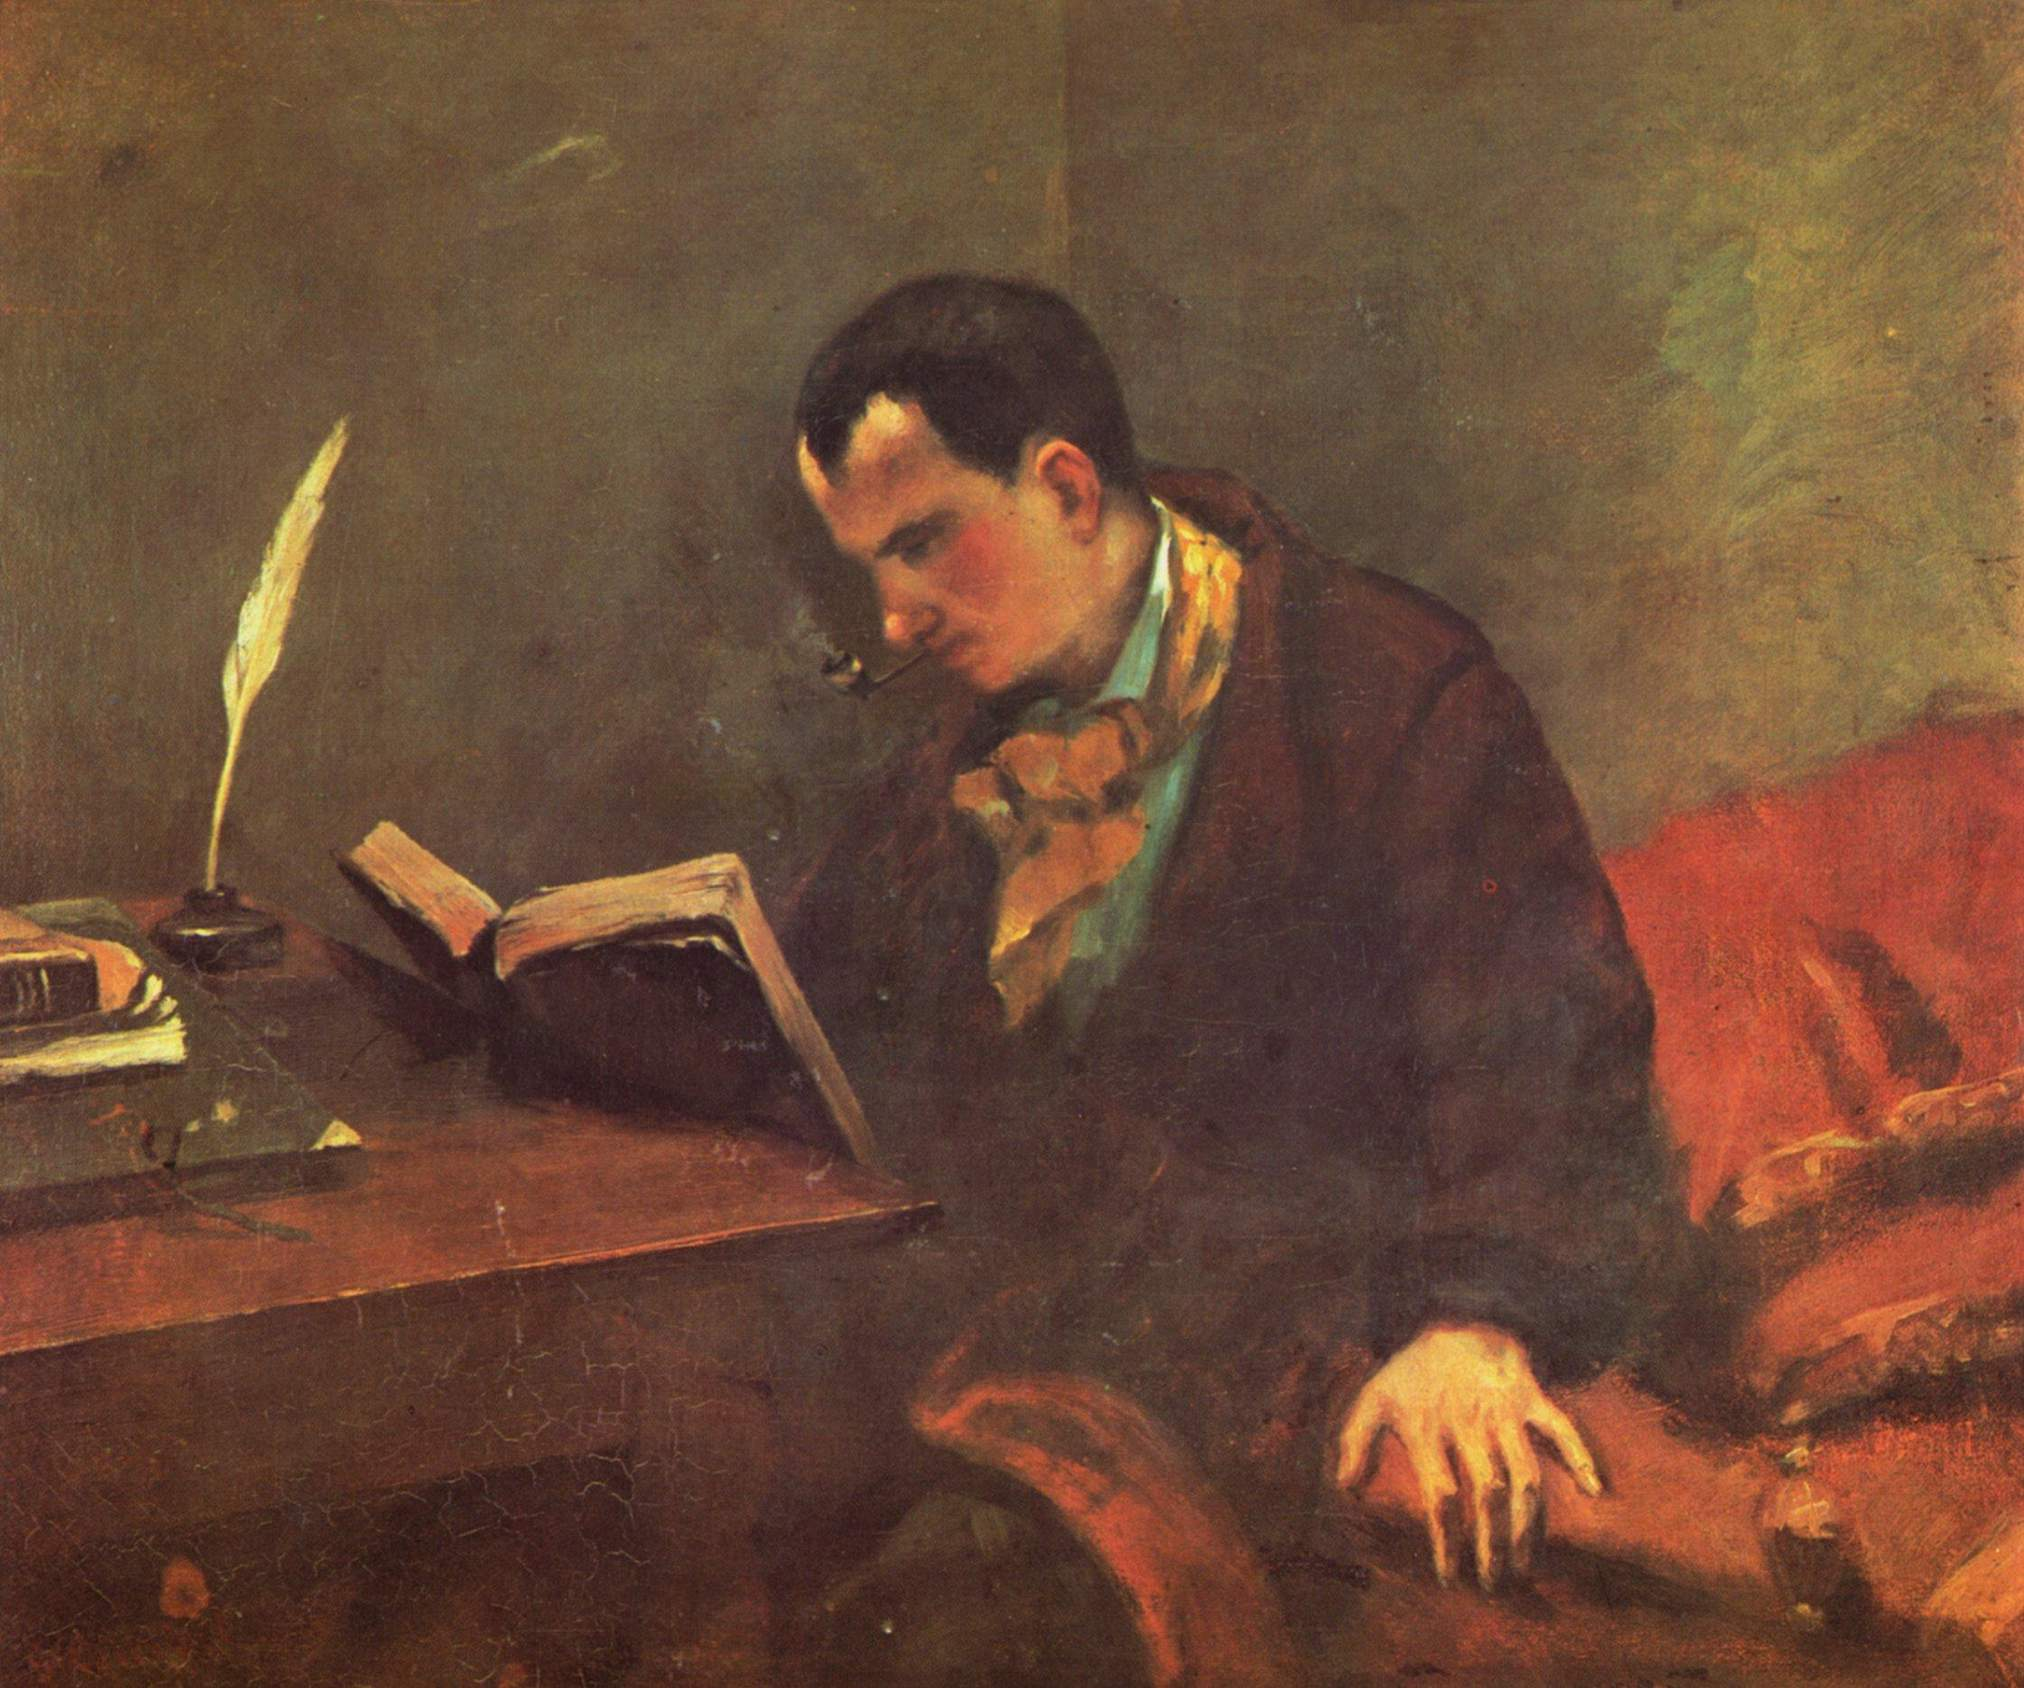
\includegraphics[keepaspectratio,width=.89\textwidth,height=.9\textheight]{Gustave_Courbet_033.jpg}
\end{myframe}

\begin{myframe}
\pictitle{La Loge de l'opéra}{Loge}{Ложа}{Constantin Guys}{Albertina, Vienna}{http://commons.wikimedia.org/wiki/File:Constantin-Ernest-Adolphe-Hyacinthe_Guys_001.jpg?uselang=ru}

\pict{Constantin-Ernest-Adolphe-Hyacinthe_Guys_001.jpg}
\end{myframe}


\begin{myframe}
\pictitle{Un bar aux Folies Bergère}{A Bar at the Folies-Bergère}{Бар в «Фоли-Бержер»}{Édouard Manet, 1882}{Courtauld Gallery, London}{http://en.wikipedia.org/wiki/File:Edouard_Manet,_A_Bar_at_the_Folies-Bergère.jpg}

\pict{Edouard_Manet,_A_Bar_at_the_Folies-Bergere.jpg}
\end{myframe}


\end{document}
